\section{Tree-to-Model Transformation with SDMs}

The next step is to specify a set of SDMs to transform our tree to an instance of our dictionary metamodel.
Take a look at the overview (Fig.~\ref{fig:moca-overview}) again and try to identify which arrow depicts exactly this \emph{tree-to-model} transformation.
Just a short comment;  all SDMs in this section depict story patterns directly in their story nodes.
Please do not take this as a \emph{best practice}, in fact we actually recommend always extracting story patterns.
It's just easier for the tutorial to fit each SDM on a single page!

\begin{enumerate}
  \item[$\blacktriangleright$]  In the code adapter project
  \texttt{DictionaryCodeAdapter}, create a \texttt{Trans\-for\-mer} class with the methods and references to the \texttt{Library} class as depicted in Fig.~\ref{fig:moca-DictionaryCodeAdapter}.\footnote{Do not forget to hold \texttt{Ctrl} when dragging the class in and to choose ``as Simple Link'' so that the class itself is added to the diagram and not an instance of it.}
  Some of the methods are for the model-to-text transformation and the corresponding SDMs shall be handled in Chapter~\ref{chap:model-to-tree}.
%\usepackage{graphics} is needed for \includegraphics
\begin{figure}[!htbp]
\begin{center}
 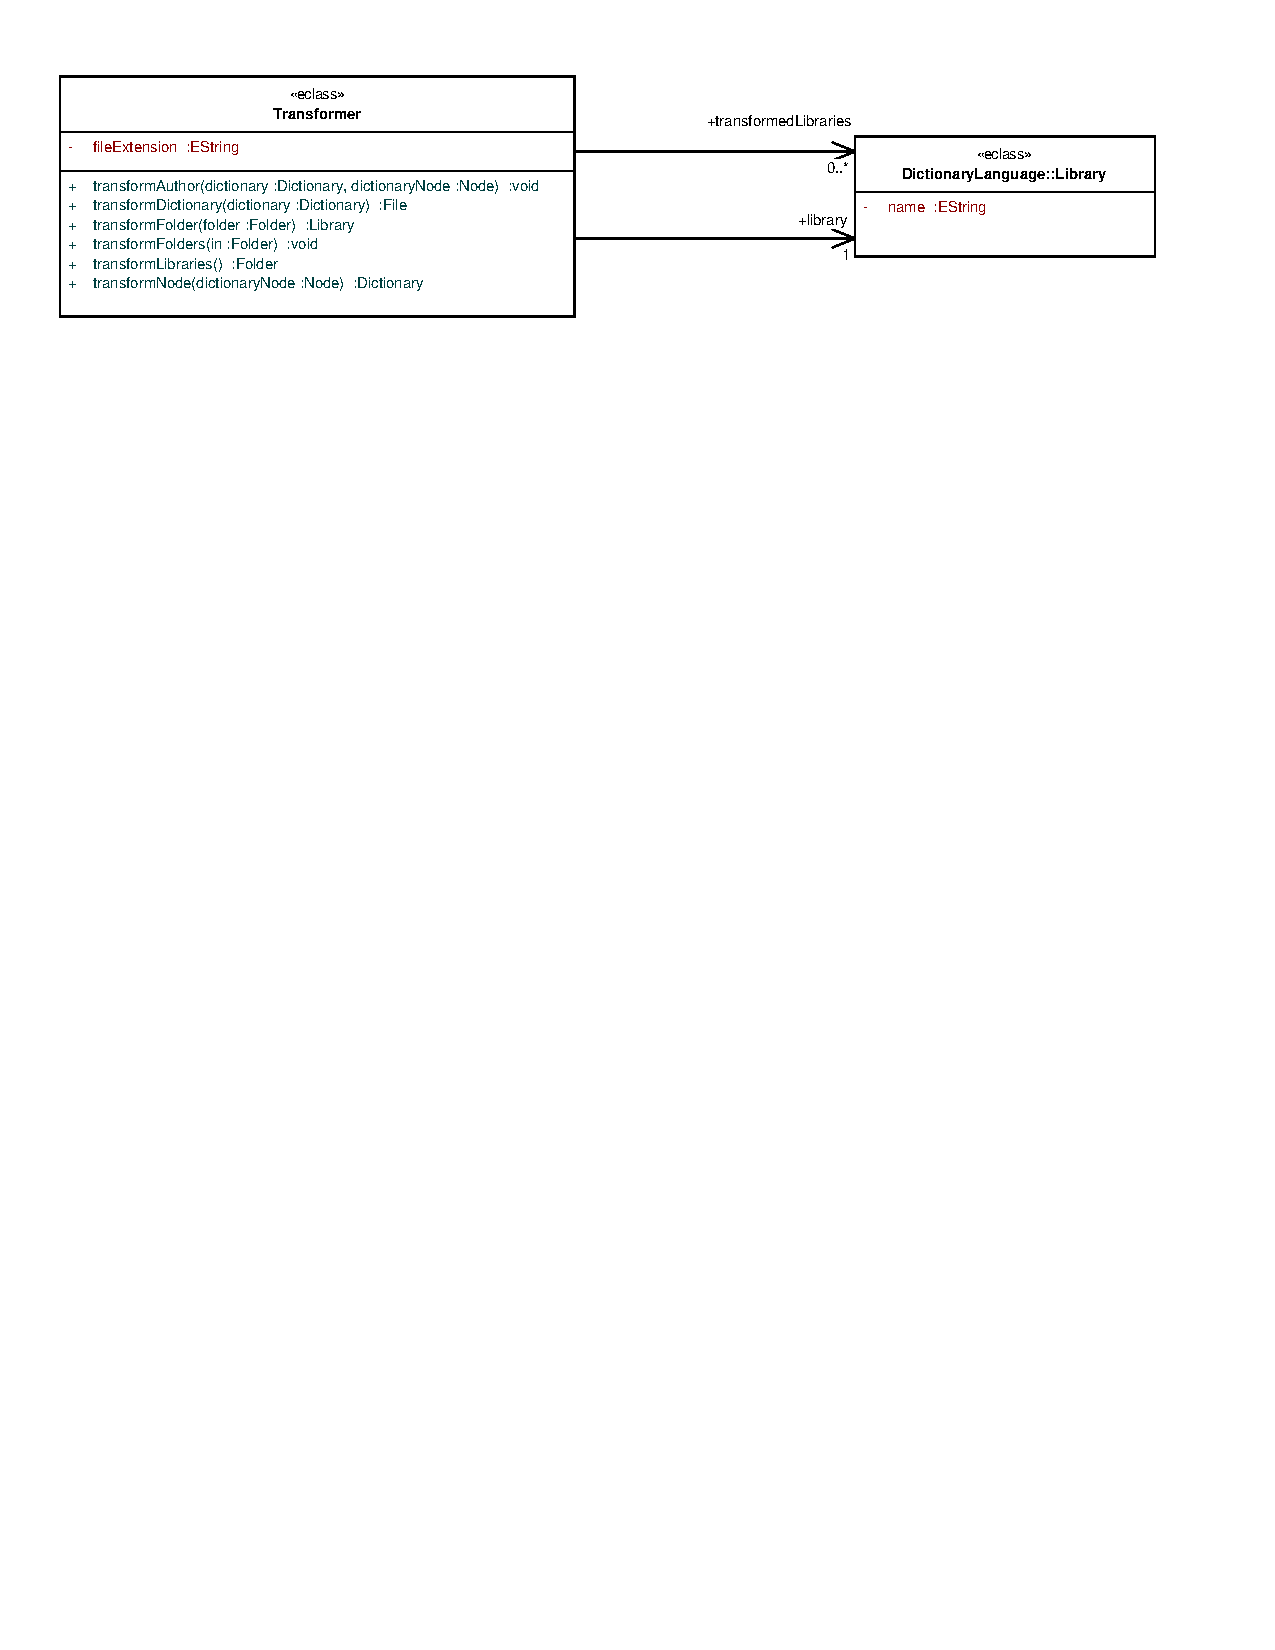
\includegraphics[width=\textwidth]{pics/moca/3MocaTreeToModel/DictionaryCodeAdapter}
  \caption{Transformer class with methods for SDMs}
  \label{fig:moca-DictionaryCodeAdapter}
\end{center}
\end{figure}
\item[$\blacktriangleright$] The first SDM \texttt{transformFolders(Folder)~:void} (Fig.~\ref{fig:moca-transformFolders}) simply iterates through all the library folders and stores the created libraries in the collection \texttt{transformedLibraries}.
%\usepackage{graphics} is needed for \includegraphics
\begin{figure}[!htbp]
\begin{center}
 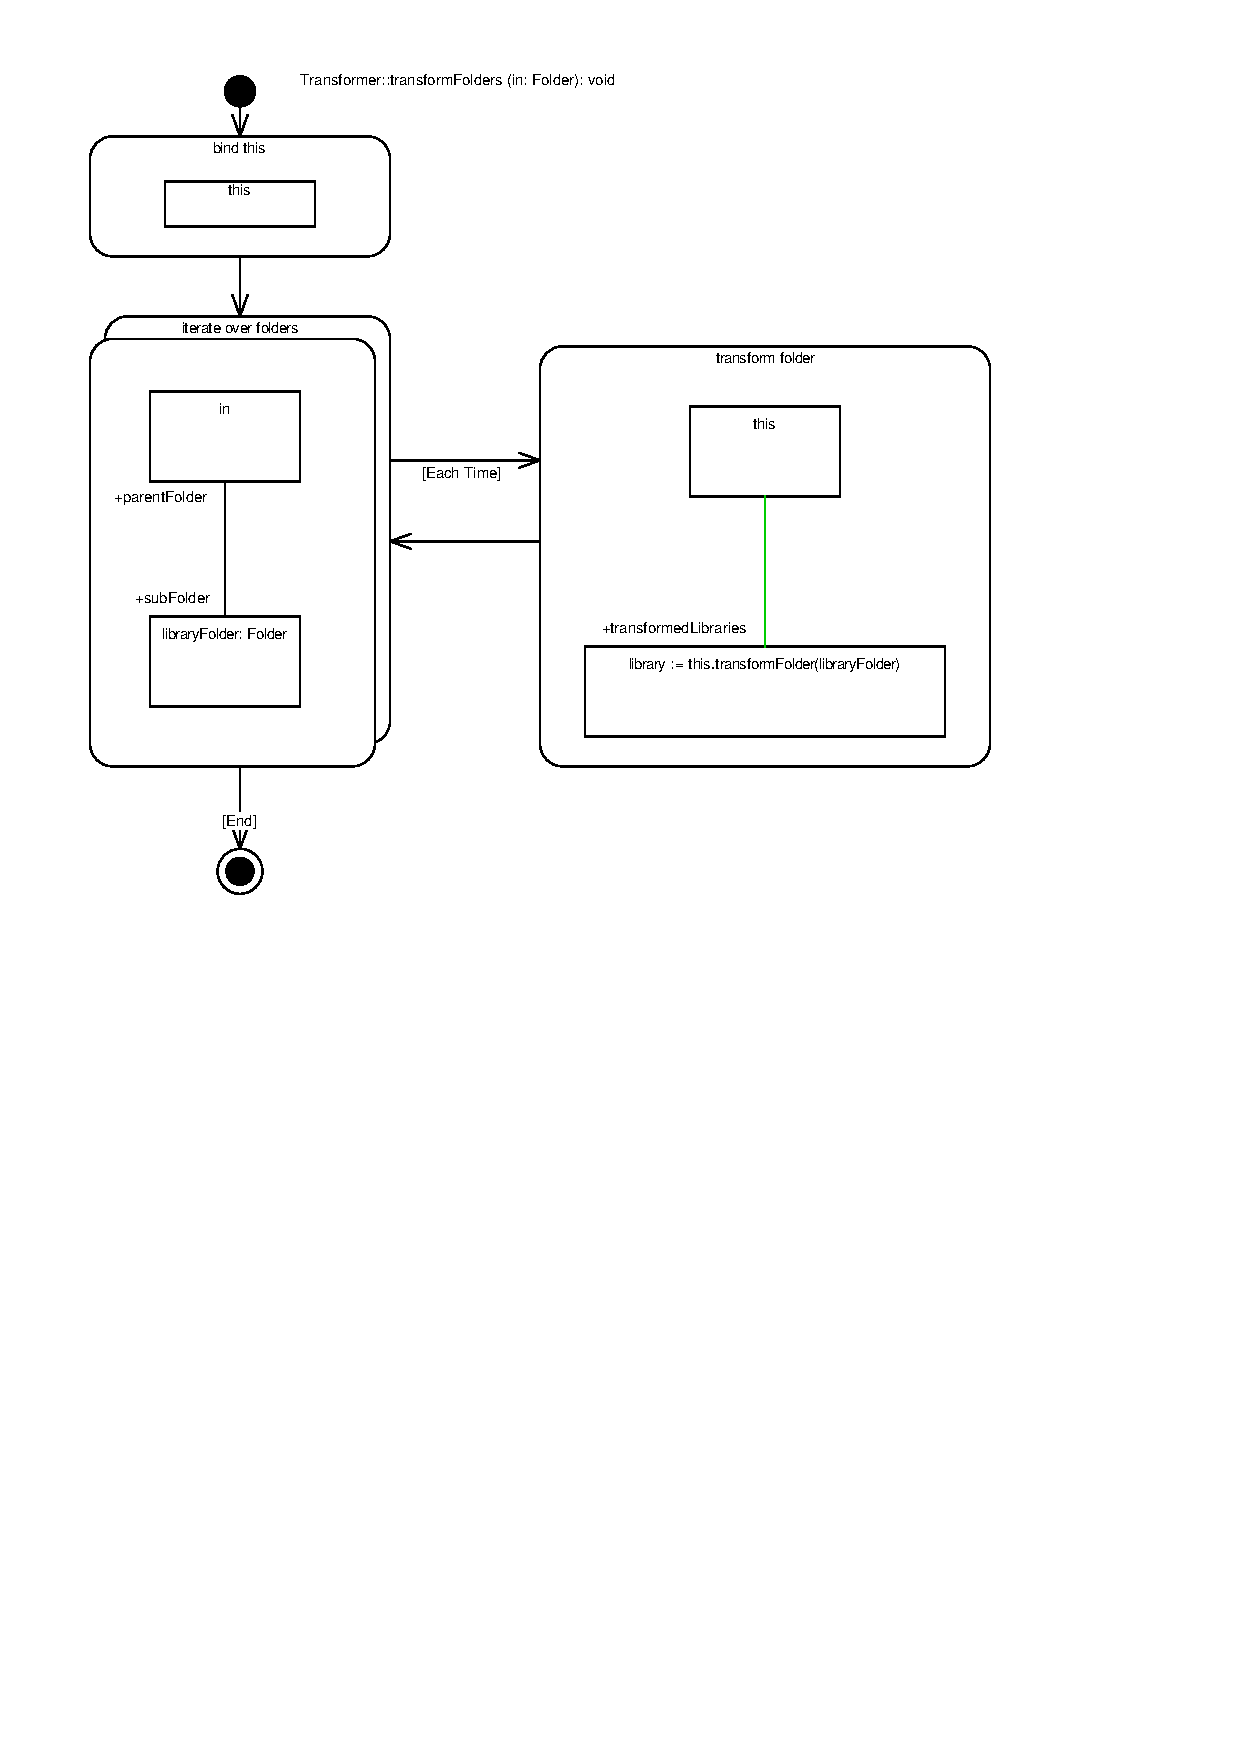
\includegraphics[width=\textwidth]{pics/moca/3MocaTreeToModel/transformFolders}
  \caption{Iterate over all subfolders of the given folder}
  \label{fig:moca-transformFolders}
\end{center}
\end{figure}
\item[$\blacktriangleright$]  \texttt{transformFolder(Folder)~:Library} (Fig.~\ref{fig:moca-transformFolder}) does the main work and creates a corresponding library with shelves for the given folder, delegating the actual creation of dictionaries to \texttt{transformNode}.
The SDM uses features that we have treated in previous chapters.
Note that the exogenous transformation is specified by simply drag \& dropping in elements from \emph{different} metamodels as required!
All dependencies are automatically added when exporting to Eclipse -- now isn't that as simple as ABC?
%\usepackage{graphics} is needed for \includegraphics
\begin{figure}[!htbp]
\begin{center}
 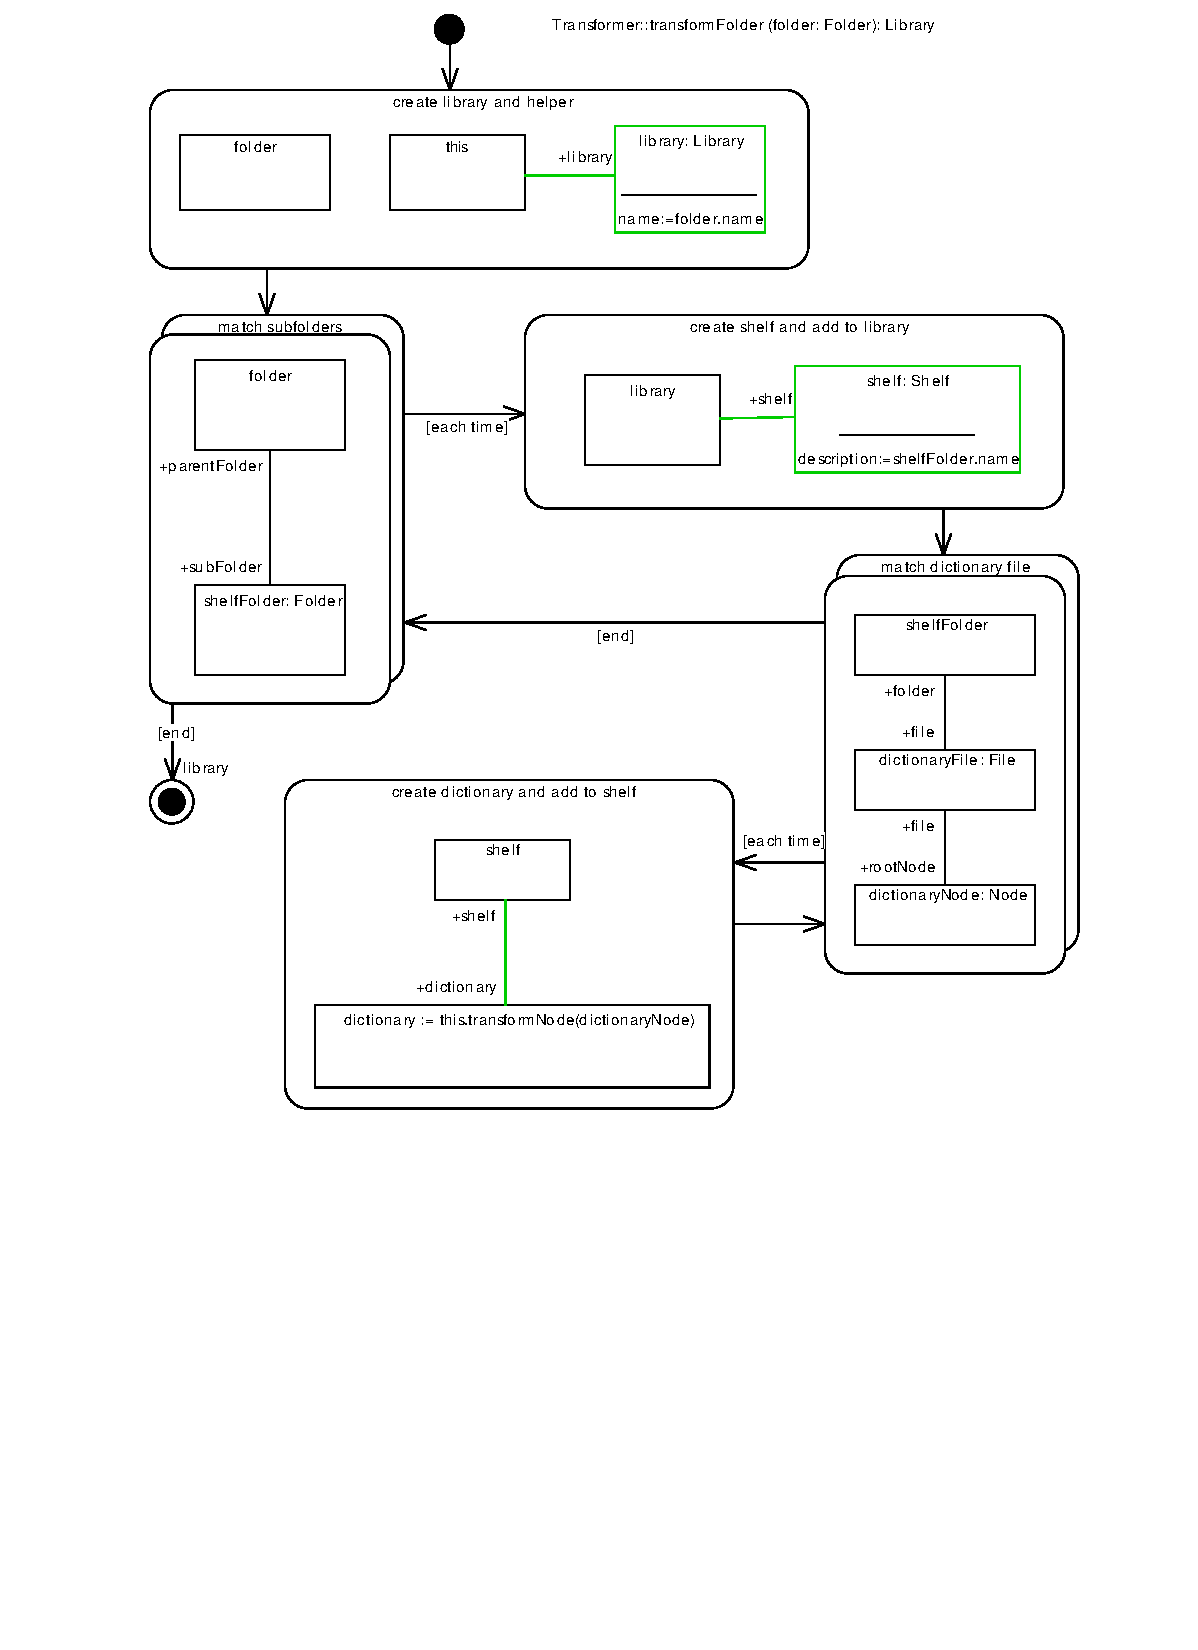
\includegraphics[width=\textwidth]{pics/moca/3MocaTreeToModel/transformFolderPrintPdf}
  \caption{Transforming the outermost folder into a library}
  \label{fig:moca-transformFolder}
\end{center}
\end{figure}

\item[$\blacktriangleright$] The next SDM, \texttt{transformNode(Node)~:Dic\-tion\-ary} (Fig.~\ref{fig:moca-transformNode}) takes a node, representing a dictionary, and builds up a dictionary object, adding entries appropriately.
It further delegates creation of authors to \texttt{transformAuthor}.\footnote{Note that multiple arguments for a MethodCallExpression \emph{cannot} be entered on a single line and separated, e.g. with a ``,'' but rather have to be chosen in the drop-down menu and entered separately, pressing \texttt{Save} each time.}
Note how \emph{indices} are used in the story node \texttt{match entry node} to decide, according to convention (how we built the tree), which node in the tree is to be interpreted as content and which as the level of the entry.
%\usepackage{graphics} is needed for \includegraphics
\begin{figure}[!htbp]
\begin{center}
 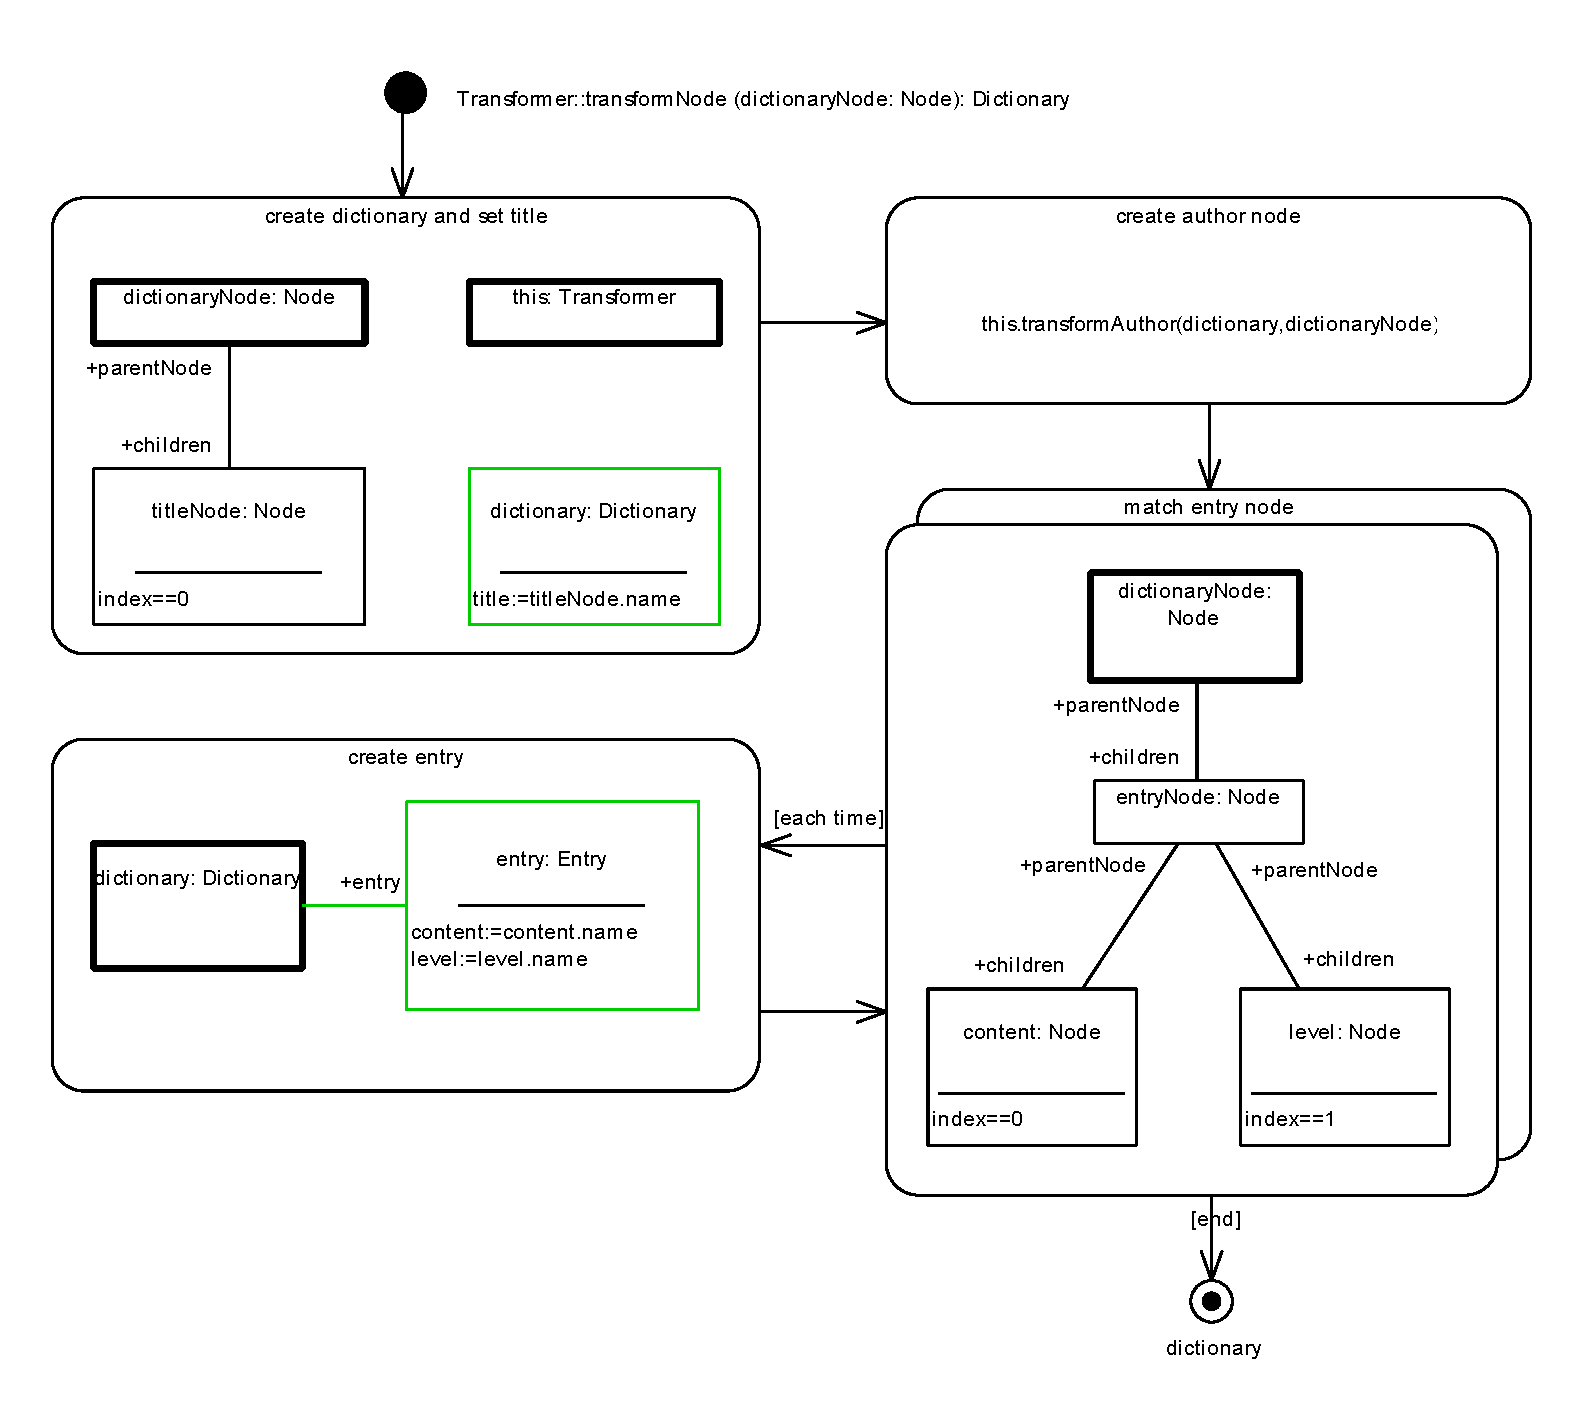
\includegraphics[width=\textwidth]{pics/moca/3MocaTreeToModel/transformNodePrintPdf}
  \caption{Creating dictionaries from dictionary nodes} 
  \label{fig:moca-transformNode}
\end{center}
\end{figure}

\item[$\blacktriangleright$] To wrap things up, create the last SDM, \texttt{trans\-form\-Author(Node)} as depicted in Fig.~\ref{fig:moca-transformAuthor}.
This SDM checks in \texttt{match author node} if the node with \texttt{index} 1 is \emph{not} an entry.
Again according to convention, this would be an author node which is optional.
If no such node exists we do not create an author and simply return.
If such a node does exist, a further complication is that the author might already be known in the library.
In order to avoid multiple, actually identical authors, the author object variable in \texttt{create author} is set to \texttt{optional} and to \texttt{create}.
\marginpar{\emph{Optional Create}} 
 
The semantics of \emph{optional create} is the following:  if a match for the object variable with the specified attribute \emph{constraints} is found, it is used.
If no match can be found then the object variable is created and the specified attribute assignments are carried out.

This is exactly how we need to handle authors -- cool right? 
%\usepackage{graphics} is needed for \includegraphics
\begin{figure}[!htbp]
\begin{center}
 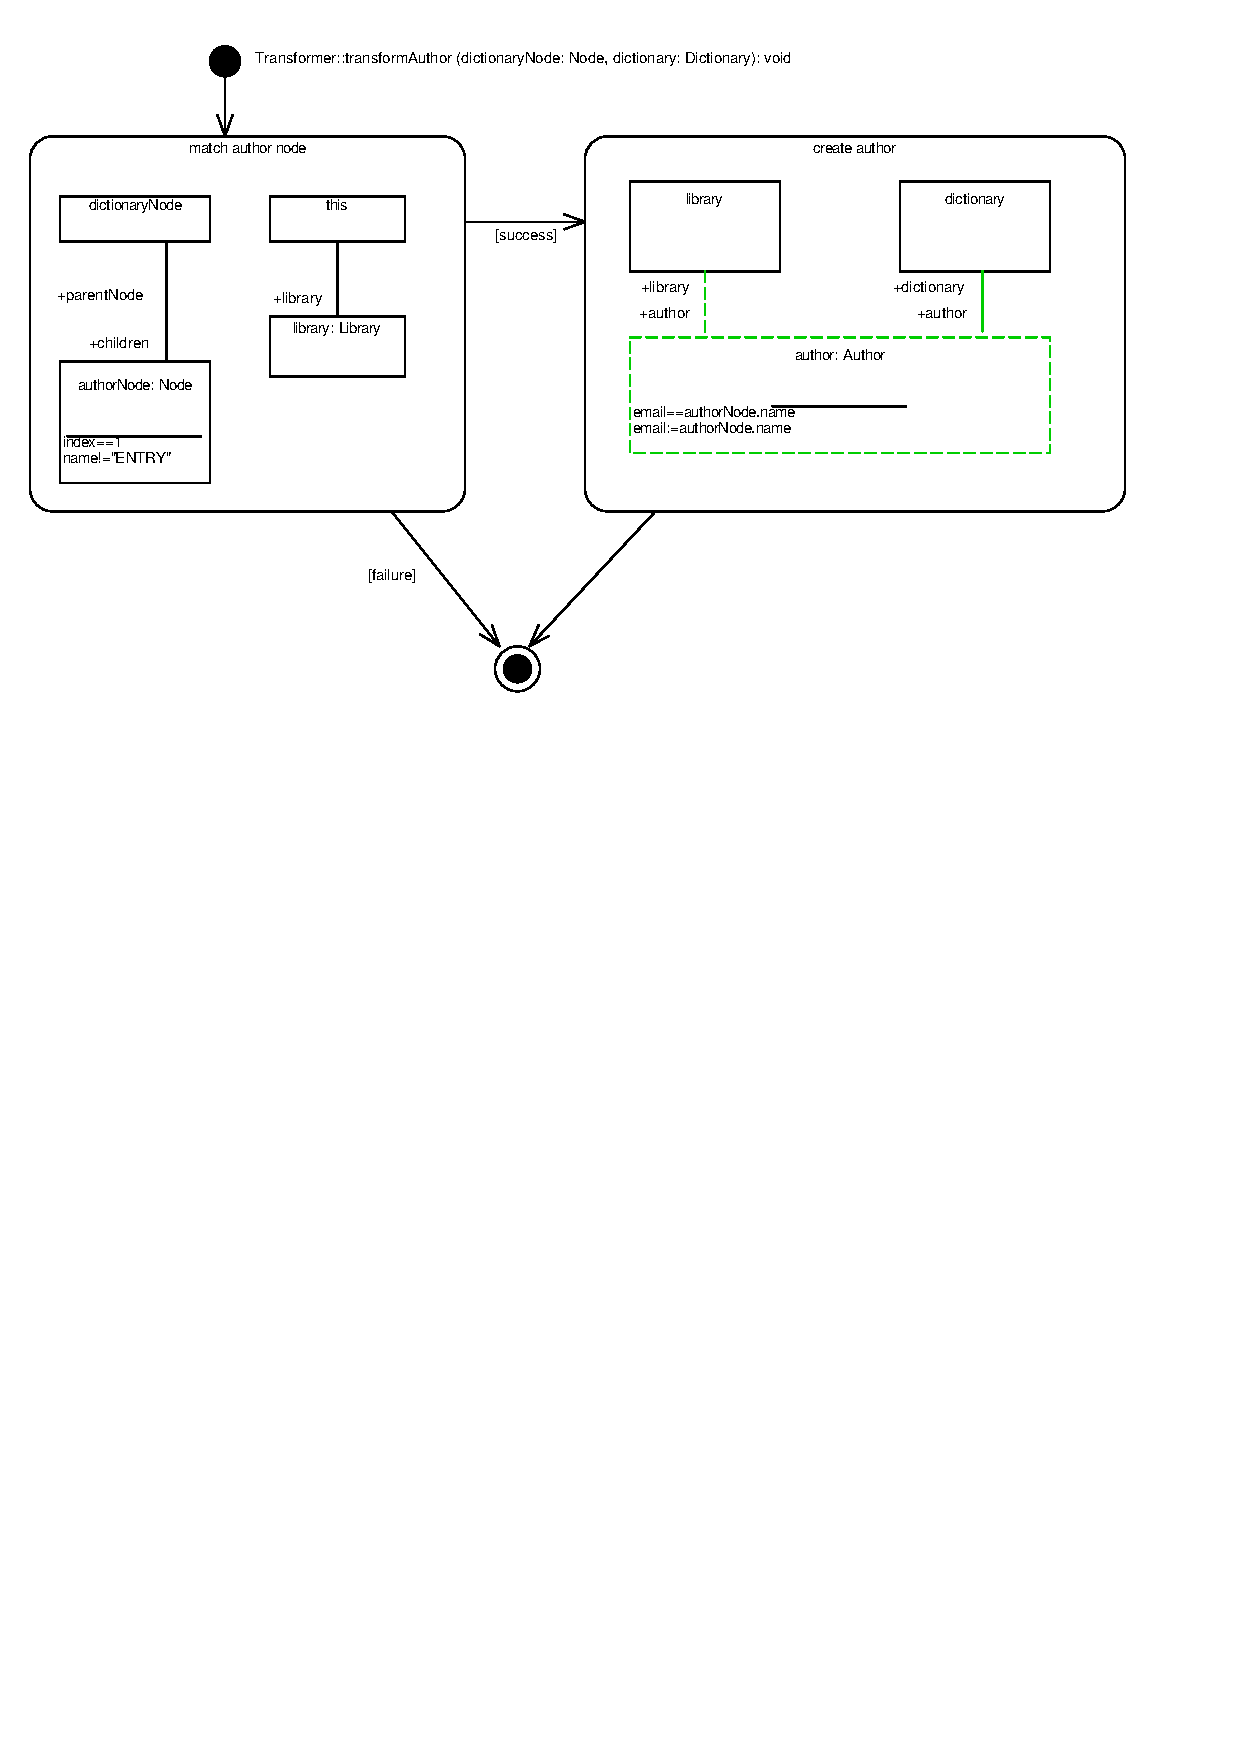
\includegraphics[width=\textwidth]{pics/moca/3MocaTreeToModel/transformAuthorPrint}
  \caption{Handling Authors}
  \label{fig:moca-transformAuthor}
\end{center}
\end{figure}

\item[$\blacktriangleright$] As a final step, open \texttt{MocaMain.java}
(Fig.~\ref{fig:moca-8-MocaMain}) and edit lines 32 -- 36 as follows:
\begin{verbatim}
// Perform tree-to-model 
Transformer transformer = DictionaryCodeAdapterFactory.
  eINSTANCE.createTransformer();
transformer.transformFolders(tree);

// Save library models
for (Library library : transformer.getTransformedLibraries())
  eMoflonEMFUtil.saveModel(MocaTreePackage.eINSTANCE, 
  	library, "instances/" + library.getName() + ".xmi"); 
\end{verbatim}
  
To see the effects of running \texttt{MocaMain.java}, refresh (\texttt{F5}) the Eclipse project to see the newly created \texttt{myLibrary.xmi} (Fig.~\ref{fig:moca-created-libary}).  
Open and inspect the library model using the reflective model browser and note especially the cross-tree references between authors and their dictionaries. 
\end{enumerate}

%\usepackage{graphics} is needed for \includegraphics
\begin{figure}[htp]
\begin{center}
  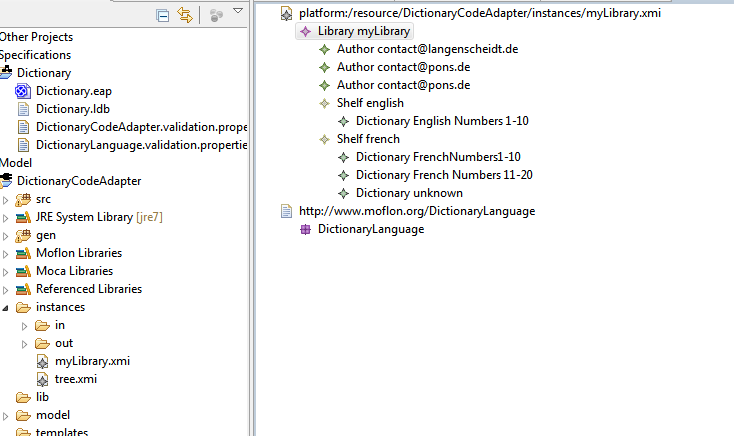
\includegraphics[width=\textwidth]{pics/moca/3MocaTreeToModel/tree_to_model_filesystem.png}
  \caption{Created library model}
  \label{fig:moca-created-libary}
\end{center}
\end{figure}